%!TEX root = ../main.tex
% file: assignment3.tex

\section{Assignment Three: Convolve Times} % (fold)
\label{sec:assignment_three_convolve_times}

In this section, we illustrate how one can use the FFT to transform a convolution into a componentwise product. This transforms the operation from $\mathcal{O}(n^2)$ to $\mathcal{O}(n \log_2(n))$. 
\\\\
We verify this order by timing how long it takes to perform convolution without FFT and then comparing that with the time it takes to perform convolution using FFT. We repeat this process a number of times using the same vectors to obtain more robust results. We also then repeat this process for various values of $n$.


\subsection{Method} % (fold)
\label{sub:methodc}

We begin by specifying a starting number of observations to test. We then create an list of observations to test by doubling the original number of observations a specified amount of times. 


\begin{lstlisting}[caption={Creating a list of n observations to test},label=lst:listobs,firstnumber=24]
# Number of iterations
r=200

# Number of observations to test
start=5
count=10
x = np.array([(2**j)*start for j in range(count+1)])
\end{lstlisting}\noindent
Next we generate random coefficient vectors for the two polynomials. Note that when performing convolution using the fftconvolve function from the \emph{scipy.signal} module, it is unnecessary to pad with zeros. This is explicitly demonstrated in the sample file \emph{convolve\_padding.py}.

\begin{lstlisting}[caption={Generating Coefficient Vectors},label=lst:coefvec,firstnumber=34]
# Generate random vectors 
a=np.array([random.randint(0,10) for i in range(1,max(x))])
b=np.array([random.randint(0,10) for i in range(1,max(x))])
\end{lstlisting}\noindent
We then repeatedly perform the convolutions without FFT using slices from the original coefficient vectors and measure the amount of time the calculation takes. To perform the convolutions, we are utilizing the convolution function from the \emph{numpy} package. We then increase the number of observations and repeat that process. Calculation times are appended to a list.

\begin{lstlisting}[caption={Convolution without FFT},label=lst:convnofft,firstnumber=48]
times1=[]

timed=timer()
for i in x:
    timed()
    for j in range(1,r):
        np.convolve(a[:i],b[:i])
    t=timed()
    times1.append(t)
\end{lstlisting}\noindent
We then repeat this process but instead performing the convolutions with FFT.

\begin{lstlisting}[caption={Convolution with FFT},label=lst:convwfft,firstnumber=62]
times2=[]

timed=timer()
for i in x:
    timed()
    for j in range(1,r):
        fftconvolve(a[:i],b[:i])
    t=timed()
    times2.append(t)
\end{lstlisting}\noindent
Lastly, to verify that the calculation times for the convolutions with FFT and without FFT are of the specified orders, we calculate the proportionality constant, $\alpha$, by finding the value that minimizes the residual sum of squares. This is used to determine what times one would expect for that order and value of $n$.
\\\\
Non-FFT:
\begin{equation}
    ExpectedTime_n=\alpha_2*n^2
\end{equation}\noindent
\begin{equation}
    \underset{\alpha_2}{\operatorname{argmin}}
    \sum_{n}(observation_n-\alpha_2*n^2)^2
\end{equation}\noindent


\begin{lstlisting}[caption={Calculating the proportionality constants for Non-FFT},label=lst:constcalc,firstnumber=77]
# Calc expected times for convolve
def residuals(alpha,observed,expected):
            return observed-alpha*expected

        
expected1 = np.array([i**2 for i in x])
observed1 = times1
p0=.001

W = leastsq(residuals,p0,args=(observed1,expected1), maxfev=100000, full_output=1)
expected_adjusted1 = [float(W[0])*expected1[i] for i in range(len(expected1))]
\end{lstlisting}
FFT:
\begin{equation}
    ExpectedTime_n=\alpha_1*n*log_2(n)
\end{equation}\noindent
\begin{equation}
    \underset{\alpha_1}{\operatorname{argmin}}
    \sum_{n}(observation_n-\alpha_1*n*log_2(n))^2
\end{equation}\noindent
\begin{lstlisting}[caption={Calculating the proportionality constants for FFT},label=lst:propcalc,firstnumber=77]
# Calc expected times for FFT
expected2 = np.array([log(i,2.0)*i for i in x])
observed2 = times2
p0=.001
W = leastsq(residuals,p0,args=(observed2,expected2), maxfev=100000, full_output=1)
expected_adjusted2 = [float(W[0])*expected2[i] for i in range(len(expected2))]
\end{lstlisting}

% subsection method (end) 

\subsection{Results} % (fold)
\label{sub:Results}

The results clearly show that convolution without the FFT and with FFT behaves as expected. For sufficiently large n, convolution with FFT is significantly less computationally intensive. 

\begin{figure}[H]
    \centering
        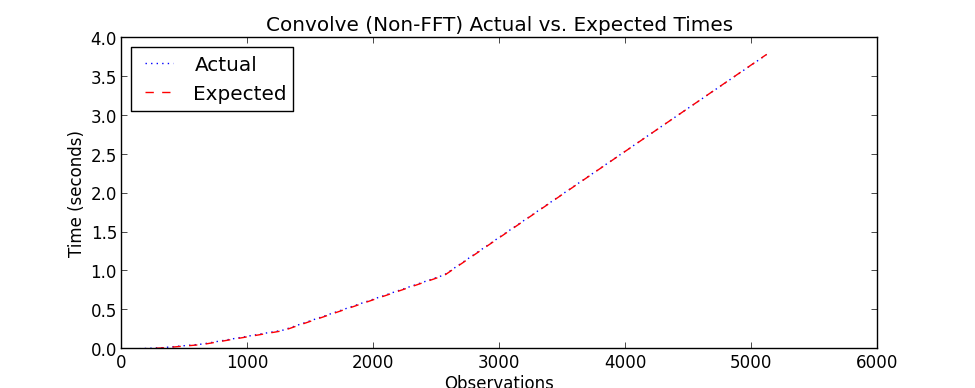
\includegraphics[width=6.5in]{./include/convolve_nonfft.png}
    \label{fig:convolve_nonfft}
    \caption{Non-FFT Actual vs. Expected Times}
\end{figure}\noindent
Figure~\ref{fig:convolve_nonfft} illustrates that the Non-FFT convolution times are as expected. It is shown that the actual times observed for the Non-FFT convolution, plus the \emph{Expected Times} calculated as previously stated. 

\begin{figure}[H]
    \centering
        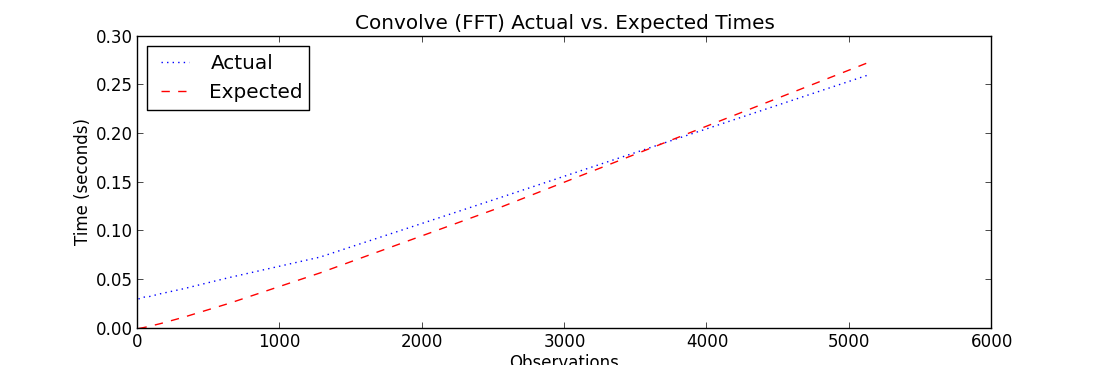
\includegraphics[width=6.5in]{./include/convolve_fft.png}
        \caption{FFT Actual vs. Expected Times}
        \label{fig:convolve_fft}
\end{figure}\noindent
Similarly, Figure~\ref{fig:convolve_fft} depicts that the FFT convolution also follows the expected trend. It is interesting to note that the plotted times do not go through the origin due to the computational overhead of these functions. However, it becomes obvious as n is large that the order is indeed $\mathcal{O}(n \log_2(n))$.

\begin{figure}[H]
    \centering
        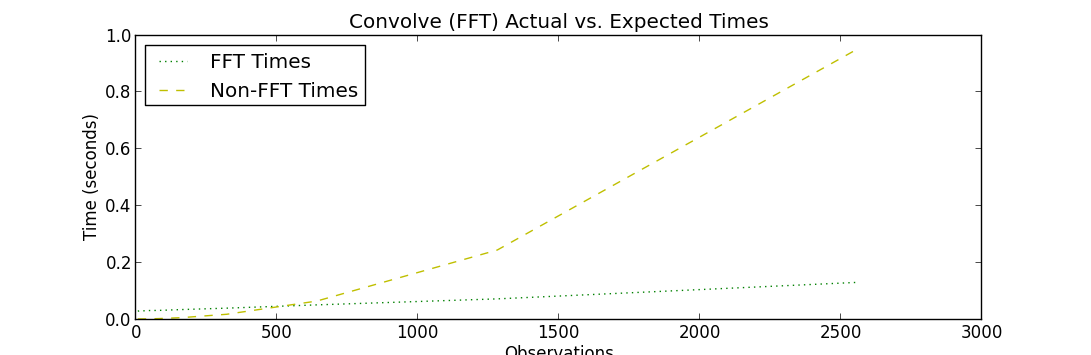
\includegraphics[width=6.5in]{./include/convolve_fft_vs_nonfft.png}
        \caption{Comparison of FFT vs Non-FFT Convolution}
        \label{fig:convolve_fft_vs_nonfft}
\end{figure}\noindent
Lastly, we examined under what conditions was the FFT faster than the Non-FFT. Figure~\ref{fig:convolve_fft_vs_nonfft} shows the two times plotted against each other. The reader should note that for small values of $n$, the Non-FFT convolution was actually faster. However, for large values of $n$, FFT convolution was significantly faster. 

% subsection results (end) 